

\subsubsection{フロアマップを用いた初期進行方向の補正}

図\ref{fig:pdr-remove-drift}の軌跡には,初期進行方向の誤差という重要な
問題が残されている.初期進行方向が誤っていると,その後の全ての推定位置が
実際の移動経路から大きく逸れることになる.この問題に対処するため,本ライブラリ
ではMapMatchCorrectorクラスを提供している.

この手法を利用するために必要な情報はフロアマップ情報である.フロアマップは
建物の構造を表す2次元の画像データとして与えられ,歩行可能な領域と
歩行不可能な領域を区別できる必要がある.図\ref{fig:floor-map}に実際の
フロアマップを示す.このマップでは灰色の部分が歩行可能領域,白色の部分が
歩行不可能領域を表している.
この手法の利用例を\ref{lst:rotate-trajectory-using-ble-fingerprint}に示す


% TODO: 2.修正関数の呼出しの部分は削除したがそれでよかったのだろうか
% TODO: 2.captionの名前は検討した方がいいかも
\begin{lstlisting}[caption={MapMatchCorrectorの使用例},label=lst:rotate-trajectory-using-ble-fingerprint,float=ht]
# フロアマップの読み込み
floor_map = FloorMap(
    floor_name="floor_5",
    floor_map_path="floor_5.png",  # 二値化された画像
    dx=0.01,  # x方向の1ピクセルあたりの距離(m)
    dy=0.01   # y方向の1ピクセルあたりの距離(m)
)

# MapMatchCorrectorの初期化
map_match_corrector = MapMatchCorrector(
    pdr_estimator=estimator,
    floor_map=floor_map
)
\end{lstlisting}

% TODO 3.どのような情報をあたえるのが重要かという所を強調したい.今回の場合はフロアマップの情報を与えるのが重要
MapMatchCorrectorクラスは,フロアマップの構造的特徴を利用して最適な初期進行方向を
推定する.この手法は,多くの屋内環境において壁や通路が直交する形で構成されているという特徴を活用している.
図\ref{fig:floor-map}に実際のフロアマップを示す.
このマップの灰色の部分が歩行可能領域であり,白色の部分が歩行不可能領域である.
図\ref{fig:floor-map}に示すような実際のフロアマップでは,
歩行可能な経路の多くが建物の主軸に沿って配置されている.

\begin{figure}[H]
	\centering
	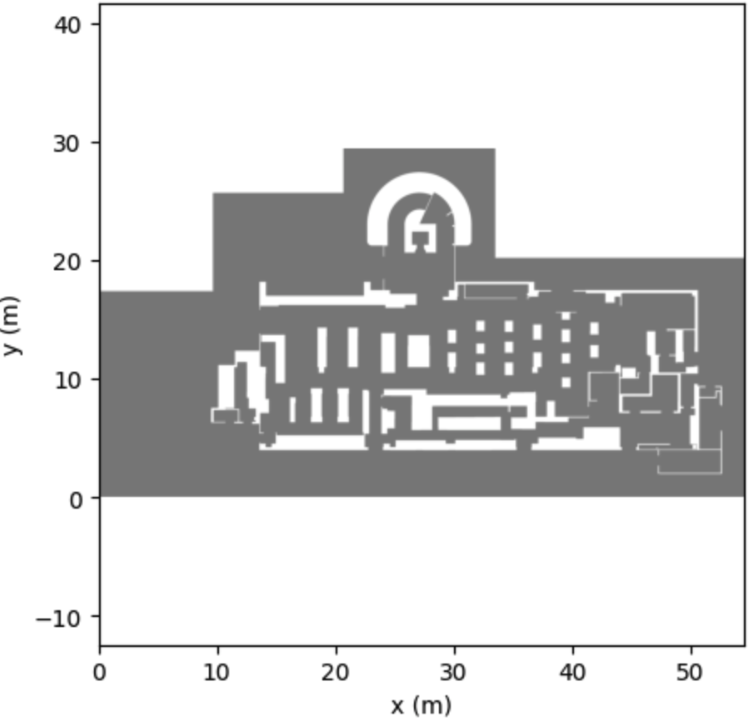
\includegraphics[width=\linewidth]{../image/floor-map.jpg}
  \caption{フロアマップ情報} \label{fig:floor-map}
\end{figure}

初期進行方向の推定は,以下の2段階のプロセスで行われる:

第一段階では,軌跡のx軸,y軸に対して平行な成分の割合を最大化する角度を探索する.
具体的には,進行方向の角度が垂直方向(90度または270度)に対して±0.1ラジアン以内,
または水平方向(0度または180度)に対して±0.1ラジアン以内の歩行ステップを平行な
成分としてカウントする.この閾値は,人間の通常の歩行では廊下や通路に対して
完全に平行でなくとも,概ねその方向に沿って歩く傾向があることを考慮して設定されている.

図\ref{fig:parallel}は,異なる回転角度での軌跡における平行成分の分布を比較したものである.
赤い点はx軸またはy軸に対して平行な成分を,青い点はそれ以外の成分を示している.
左側の例では平行な成分の割合が少なく,軌跡が建物の主軸に対して斜めに配置されている.
一方,右側の例では平行な成分の割合が多く,軌跡が建物の構造とよく整合している.
このように,平行成分の割合を分析,建物の主軸に整合する可能性の高い
角度を特定できる.ただし,この情報だけでは4つの候補角度(0度,90度,180度,
270度)のうち,どの角度が最適であるかを一意に決定するできない.
% TODO:1.ここよく考える最初から90,180,240,270度なの決まってないかな?.
% じゃあ最初から90,180,240,270度に回転させたらって思ったけど,どこを回転の基準にするのかわからないから無理そう?

\begin{figure}[H]
	\centering
	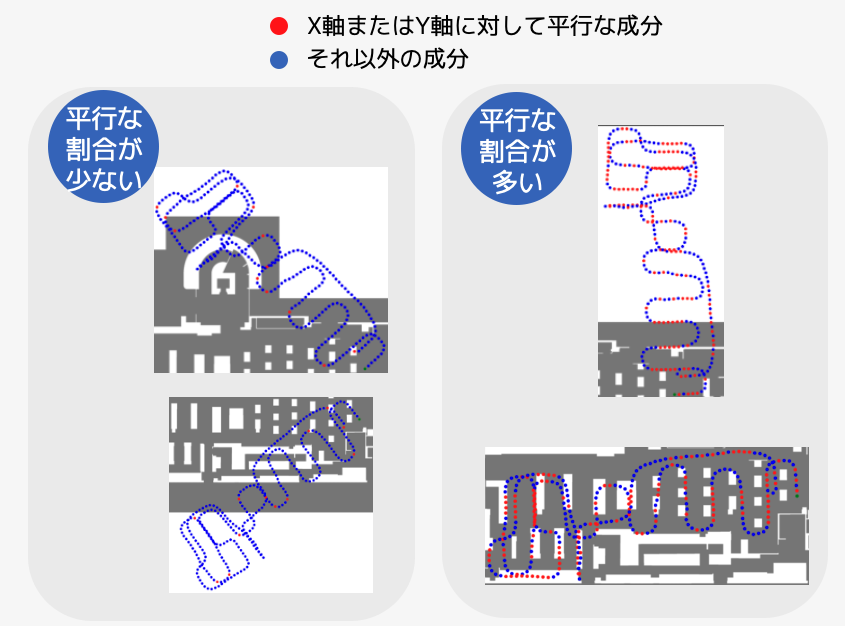
\includegraphics[width=\linewidth]{../image/parallel.jpg}
	\caption{x軸とy軸に対して平行な成分の割合}    \label{fig:parallel}
\end{figure}

第二段階では,フロアマップ上の歩行可能領域の情報を活用する.
具体的には,各候補角度で軌跡を回転させ,その軌跡上の点がフロアマップ上で歩行可能な
領域に含まれる割合を計算する.

図\ref{fig:pdr-rotate}は,この補正処理を適用した結果を示している.
補正後の軌跡は建物の構造に整合し,正解軌跡により近い形状となっている.
この手法は,特に廊下や部屋が格子状に配置された一般的なオフィスビルなどの
環境で効果的である.

\begin{figure}[H]
	\centering
	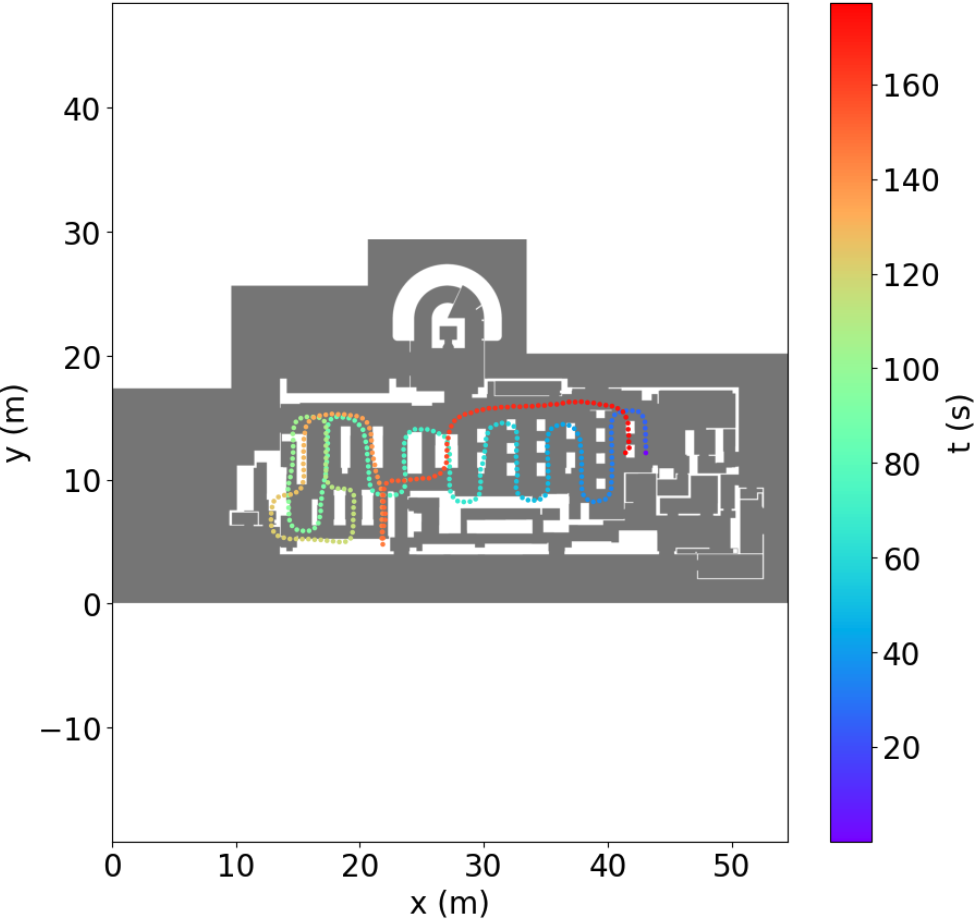
\includegraphics[width=\linewidth]{../image/pdr-rotate.jpg}
	\caption{初期進行方向の補正後の軌跡}    \label{fig:pdr-rotate}
\end{figure}



